\section{Durchführung}
\label{sec:Durchfuehrung}
\subsection{Charakteristische Strahlung von Kupfer}
Aus den Kupfer Messwerten bildet sich:
\begin{figure}[H]
    \centering
    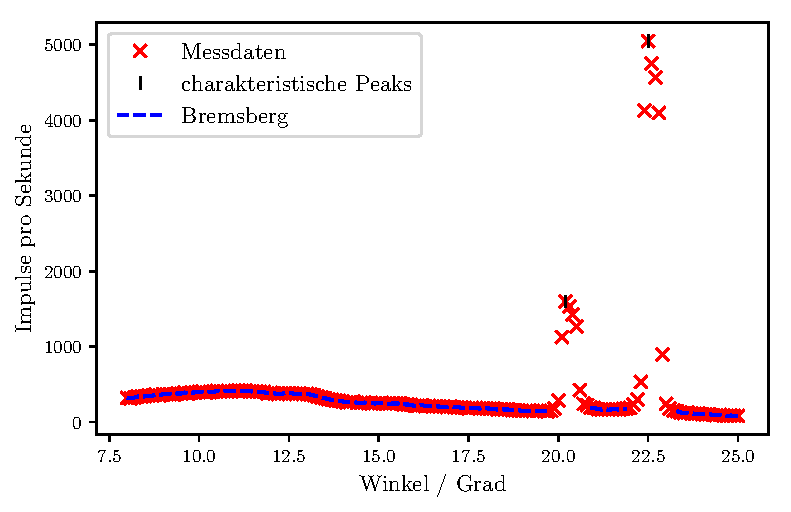
\includegraphics[width=0.7\textwidth]{plots/CU_Spektrum.pdf}
    \caption{Kupfer Emissionsspektrum mit Peaks und Bremsberg}
    \label{fig:CU_Spektrum}
\end{figure}
Mit den Peaks bei 1599 Impulsen pro Sekunde bei 20,2° und 5050 Impulsen pro Sekunde bei 22,5°.
Über die abgelesenen Winkel an den Peaks lassen sich nun die entsprechenden Energien berechnen.


\subsection{Compton Wellenlänge}
Es wird die Transmission von Aluminium gemessen.
\begin{figure}[H]
    \centering
    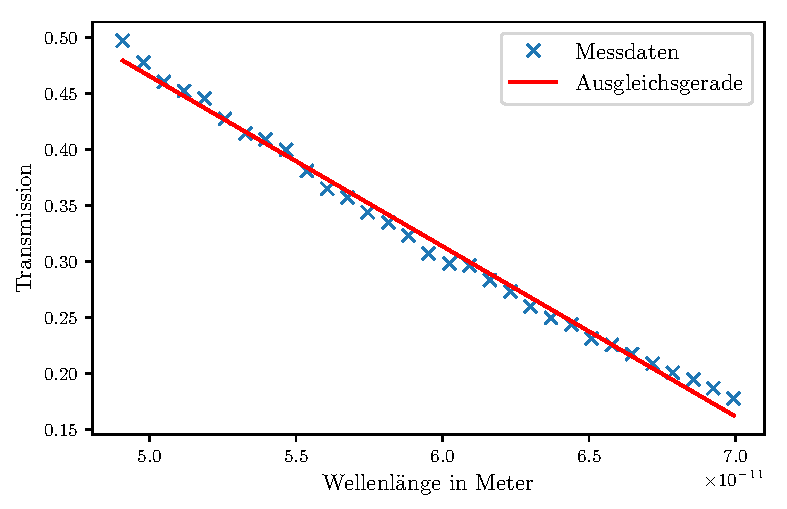
\includegraphics[width=0.7\textwidth]{plots/Transmission.pdf}
    \caption{Transmission von LiF in Abhängigkeit von der Wellenlänge}
    \label{fig:Transmission}
\end{figure}